\documentclass[conference]{IEEEtran}
\IEEEoverridecommandlockouts
% The preceding line is only needed to identify funding in the first footnote. If that is unneeded, please comment it out.
\usepackage{cite}
\usepackage{amsmath,amssymb,amsfonts}
\usepackage{algorithmic}
\usepackage{float}
\usepackage{graphicx}
\usepackage{textcomp}
\usepackage{xcolor}
\usepackage{listings}
\usepackage{balance}
\usepackage[hidelinks]{hyperref}
\def\BibTeX{{\rm B\kern-.05em{\sc i\kern-.025em b}\kern-.08em
    T\kern-.1667em\lower.7ex\hbox{E}\kern-.125emX}}

\DeclareGraphicsExtensions{.png,.PNG,.tiff,.tif,.jpeg,.jpg,.JPG,.JPEG,.gif}
\graphicspath{ {./images/} }
%\definecolor{lstgray}{gray}{0.95}
\lstset{%
	%backgroundcolor=\color{lstgray},
	stepnumber=2,
	basicstyle=\footnotesize,%
	showspaces=false,showstringspaces=true,%
	language=SQL,%
	numbers=none,tabsize=4,breaklines%
}

\begin{document}
\title{Software Defined Radio and its Applications
}

\author{\IEEEauthorblockN{Julian Janisch}
	\IEEEauthorblockA{\textit{FH OÖ Campus Hagenberg, Mobile Computing}\\
		Softwarepark 106/14\\
		4232 Hagenberg im Mühlkreis, Austria\\
		s1710237010@students.fh-hagenberg.at}
	\and
	\IEEEauthorblockN{Alexander Kemptner}
	\IEEEauthorblockA{\textit{FH OÖ Campus Hagenberg, Mobile Computing}\\
		Softwarepark 106/9\\
		4232 Hagenberg im Mühlkreis, Austria\\
		s1710237015@students.fh-hagenberg.at}
}

\maketitle

\begin{abstract}

\end{abstract}

\begin{IEEEkeywords}
SDR, antenna, signal processing, ADS-B, NOAA, replay attack 
\end{IEEEkeywords}

\section{Introduction} %Julian
%Allgemein: 
% - Was ist SDR?
% - erhältliche Hardware: HackRF, SDRplay, RTL-SDR, Airspy, LimeSDR, FunCube
%   von wem kommt er? Was kostet er? Unterschiede/Möglichkeiten?

\subsection{What is SDR?}
A software defined radio system is a radio transmission system that heavily relies on software instead of analog hardware~\cite{Heuberger2017}.\\
In case of a transmitter, it takes data as an input (source), performs a sequence of operations via software on this data, converts it to an analog signal (with the help of an DAC) and transmits it wirelessly through its radio frequency (RF) frontend. The receiver performs the same tasks in reverse order (with an ADC), finally outputting the same data on it's sink~\cite[5pp]{wyglinski2018software}.
\begin{figure}[H]
	\centering
	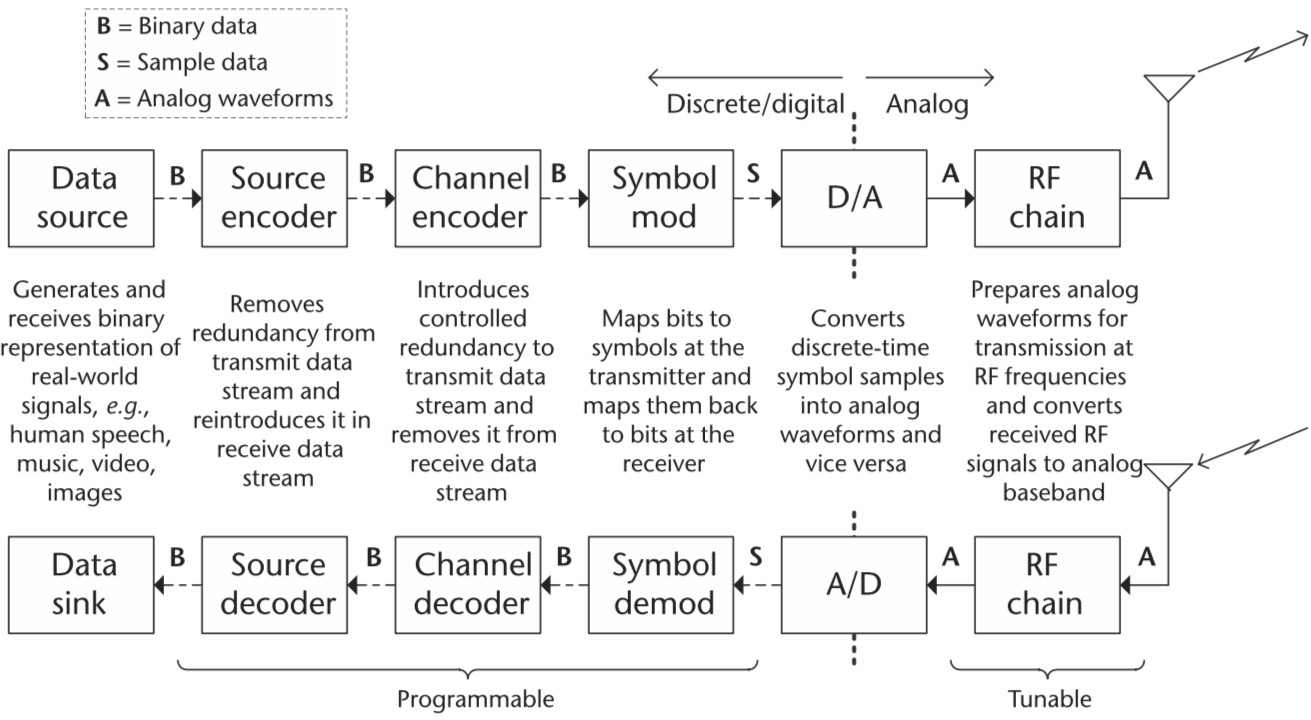
\includegraphics[width=0.5\textwidth]{forEngineers_SDR_structure}
	\caption{The structure of an SDR. Most of the processing is done on the digital side, the D/A and A/D converters are at the very end/beginning of the chain.}
\end{figure}
In the diagram, the blocks marked as programmable can be implemented in software or programmable logic~\cite[5p]{wyglinski2018software}. This makes it possible to build highly generic RF hardware that can be used for different tasks~\cite[4p]{wyglinski2018software}.\\ 
The digital processing needs to be done on an IC suited for the tasks. Commonly used parts include~\cite[3p]{Heuberger2017}:
\begin{itemize}
	\item FPGAs and ASICs for sample rate conversions
	\item Digital signal processors (DSPs) for expensive computations in the demodulator
	\item Microcontroller units (MCUs) or CPUs for all other tasks
\end{itemize}
\subsection{In this paper}
In this paper, we will present applications using inexpensive SDR hardware.\\
First, we will show the hardware we used for our experiments. Afterwards, we will present software packages available to use with SDR receivers on the different platforms. Finally, we will discuss different applications using SDRs: receiving air traffic transmissions, weather satellite images and performing replay attacks.

\section{Hardware}
There is various hardware on the market for software defined radio receivers and transmitters (HackRF, SDRplay, RTL-SDR, Airspy, LimeSDR, FunCube, etc.). The software defined radios we used were:
\begin{itemize}
	\item HackRF One - for data transmitting and receiving
	\item RTL-SDR - for data receiving
	\item SDRplay - for data receiving
\end{itemize}

\subsection{HackRF One}
Compared to the other Software Defined Radios of our list, the HackRF One with a price of around 300€ is the most expensive. But it has several advantages: It provides a very high operational bandwidth (from 30MHz to 6GHz) with an instantaneous bandwidth of 20MHz. (Instantaneos bandwidth = It can acquire 20MHz of RF spectrum around the chosen center frequency in real-time without a re-tuning of the oscillator) \cite[Kap. 2.5]{Mishra2014} The HackRf is not only able to receive radio signals, but also to transmit them. Radio signals between 30MHz and 6GHz (e.g. Signals from remote controls of wireless sockets) can be recorded and afterwards sended again. So it can also be used to perform replay attacks (see section \ref{replayattack}).  \\

\subsection{SDRplay}
In order to receive radio signals we also ordered an SDRplay (Type RSP1). This receiver covers the RF spectrum from 1kHz to 2GHz. The SDRplay ships with  a lot of software support (HDSDR, SDR Console, Cubic SDR and SDRuno), hence is very easy to setup. The instantaneous bandwidth is 10MHz and there are several preselection filters built in for better receiving-results. To provide more accuracy the SDRplay uses a 14-Bit ADC (RTL-SDR uses only 8-Bit).
\cite{sdrplay}
\\
\subsection{RTL-SDR}
This is the cheapest product on our list.(It did cost about 30€) The RTL-SDR is a USB-dongle which is capable of receiving radio signals  between 500kHz and 1,75GHz.  The  usage of these dongles started years ago from mass produced DVB-T TV Tuners. Because of an easy accessible chipset (RTL2832U) those tuners could be converted into wideband software defined radios (trough custom software drivers). This discovery made the access to the radio spectrum much cheaper. \cite{rtl-sdr}

\section{Software} %Alexander
%GNU Radio Companion
%CubicSDR
%GQRX
%command line tools
%SDR#
%sdrangel
% - Betriebssystem/von wem kommts/Lizenz/Funktionen/Backend
% - Was ist ein Waterfall-Diagramm?
\subsection{GNU Radio and the GNU Radio Companion}
GNU Radio is a signal processing software and software development toolkit available for Linux, OS X and (with less support available) Windows~\cite{Gnu19FAQ}\cite{Gnu19What}. It is licenced under GPLv3 or later~\cite{Gnu19FAQ}.\\
The desired signal processing steps are laid out as blocks that are connected to each other. End user applications are written using Python, while the performance-critical backend is written in C++.\\
The GNU radio companion is a GUI for GNU Radio which aids in building these blocks through drag-and-drop, comparable to Simulink~\cite{Gnu19FAQ}.\\
\balance
\begin{figure*}
	\centering
	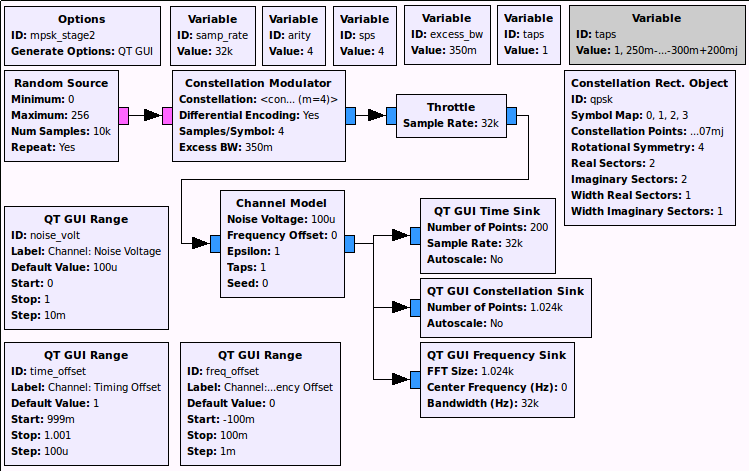
\includegraphics[width=0.8\textwidth]{gnuradio_example_flowgraph}
	\caption{An example flowgraph in GNU Radio Companion~\cite{Gnu19Example}}
\end{figure*}

\subsection{GQRX}
GQRX is a graphical frontend for GNU Radio offering an FFT plot and waterfall graph, hardware abstractions for various SDR devices to set frequency and other settings and multiple demodulators.\\
The received data can be digitally filtered and recorded to a file~\cite{GQRX19Home}.
\begin{figure}[H]
	\centering
	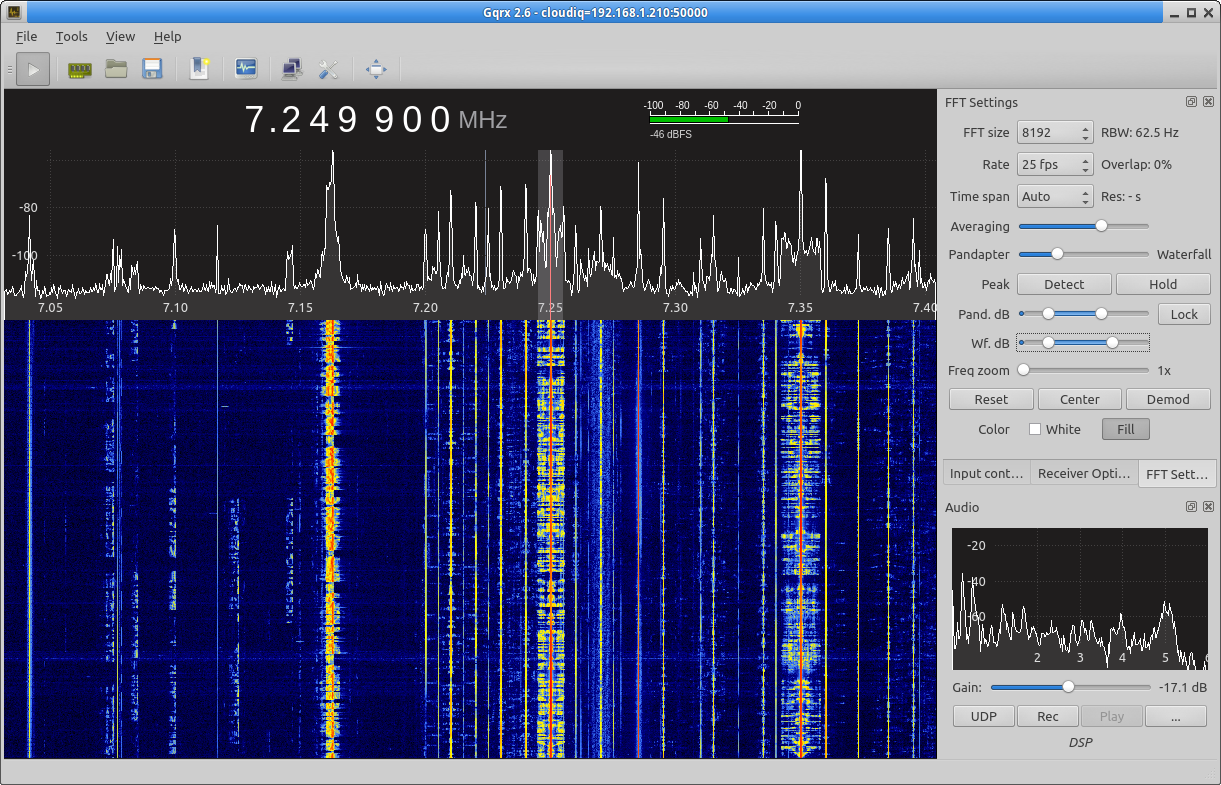
\includegraphics[width=0.5\textwidth]{gqrx_main_window}
	\caption{GQRX main window~\cite{GQRX19Home}}
\end{figure}

\subsection{SDR\#}
SDR\# (SDR sharp) is developed at Airspy for their Airspy SDRs, but can also be used with other SDRs like the RTL-SDR.\\The main software package is available for Windows only, while the "Spy Server", a program that allows streaming of the signal to clients, is available for Linux on x64/x86 and ARM (Raspberry Pi, Orange Pi).\\
The functionality can be expanded with third-party plugins~\cite{SDRsharp19Download}.

\section{ADS-B}
%Was ist ADS-B
%Wie funktioniert die Codierung?
%Welche Frequenzen gibt es? Welche Antenne wird benötigt?
%Welche Software gibt es/wie funktioniert der Workflow (hackrf_transfer/sox/dump_1090)
%Ergebnisse/Screenshots/flightradar24 Vergleich
\subsection{What is ADS-B?}
Automatic Dependent Surveillance Broadcast is a system in air traffic control for transmitting flight data (location, \ldots) from an aircraft to air traffic control stations.\\
It should replace radar as the primary tracking mechanism because of its higher precision needed in modern, densely populated air space~\cite{strohmeier2014realities}.
\subsection{Objective}
In this experiment, we want to capture and visualise the ADS-B messages sent by airplanes in our area.
\subsection{Frequencies}
Two standards with different frequencies are in use: Universal Access Transceiver (978 MHz) and 1090 MHz extended squitter (1090ES). The latter is more common in commercial aircraft, as it can be used with hardware already fitted for a previous communication standard (mode S)~\cite{strohmeier2014realities}.
\subsection{Antennas}
For our experiments, we used a monopole antenna specifically designed for ADS-B on 1090 MHz. It was sourced on Amazon for € 10,56.
\subsection{Workflow}
We used an HackRF SDR receiver for our experiment. Data was captured using the HackRF command line tool \lstinline|hackrf_transfer|. The full command used was
\begin{lstlisting}
hackrf_transfer -r - -f 1090000000 -s 2000000 -p 0 -a 0 -l 40 -g 62
\end{lstlisting}
\begin{enumerate}
	\item -r: receive data
	\item ~-: output to stdout
	\item -f: frequency in Hz
	\item -s: sample rate in samples per second
	\item -p: antenna port power (disable)
	\item -a: receiver and transmitter RF amplifier (disable)
	\item -l: receiver end low noise amplifier gain in dB
	\item -g: receiver end baseband amplifier gain in dB
\end{enumerate}
The output of \lstinline|hackrf_transfer| was then piped into SoX, an audio processing application~\cite{SoX19}. This was necessary because the hackrf uses signed bytes, while the next application expects unsigned bytes. The full command was~\cite{Medium19ADS-B}:
\begin{lstlisting}
sox --rate 2000000 --channels 1 --type sb - --type ub -
\end{lstlisting}
\begin{enumerate}
	\item --rate: the sample rate
	\item --channels: number of channels
	\item --type: type of input (signed byte)
	\item -: read from stdin
	\item --type: type of output (unsigned byte)
	\item -: write to stdout
\end{enumerate}
SoX is licenced under the GPL and is available on \url{sourceforge.net}.\\
To decode and visualize the received data, we used dump1090. It can output the data on the console and on a website running on localhost. It is available on GitHub under a BSD licence~\cite{dump109019Github}. The command used was:
\begin{lstlisting}
dump1090 --ifile - --net --interactive
\end{lstlisting}
\begin{enumerate}
	\item --ifile -: input file, read from stdin
	\item --net: enable networking
	\item --interactive: show interactive data on console
\end{enumerate}
Alternatively, the flightaware fork of dump1090 has built-in support for RTL-SDR dongles~\cite{Github19dump1090-fa}. It can be started with
\begin{lstlisting}
dump1090 --interactive
\end{lstlisting}
Both sources, RTL-SDR and HackRF produce an output similar to the one shown in figure \ref{fig:dump1090screenshot}. In interactive mode, one row corresponds to one aircraft. Rows are updated continuously and deleted if no messages from this aircraft were received in the last 60 seconds. Decoded fields are, among others, flight number, squawk code, altitude, coordinates, speed, heading, number of messages received and signal strength~\cite{dump109019Github}. One can see that just after the one-minute-mark, some aircraft are approaching 2,000 messages. 
\begin{figure}
	\centering
	\caption{Output of dump1090 on 23rd June, 20:13 in Hagenberg/Mühlkreis} \label{fig:dump1090screenshot}
	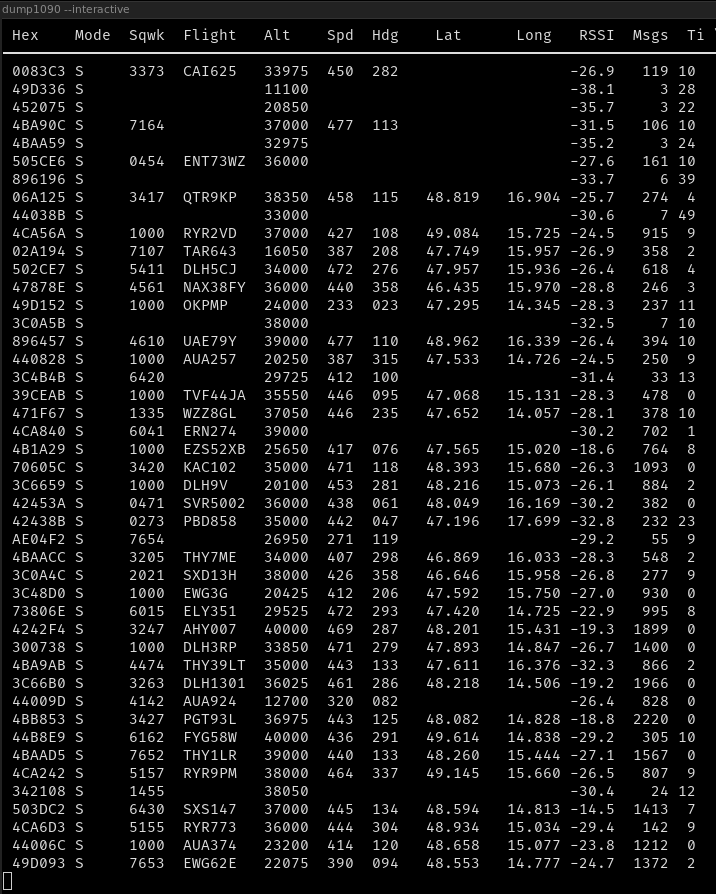
\includegraphics[width=0.5\textwidth]{dump1090_screenshot}
\end{figure}

\section{NOAA APT} %Alexander
%Was ist NOAA
%Wie funktioniert die Codierung?
%Welche Frequenzen gibt es? Welche Antenne wird benötigt?
%Bau der Antenne (verschiedene Typen: V-Dipol, QFH, ...)
%Welche Software gibt es/wie funktioniert der Workflow
%Ergebnisse/Screenshots
\subsection{What is NOAA?}
The \textit{National Oceanic and Atmospheric Administration} is an organisation of the US government producing, among other things, weather forecasts~\cite{NOAA19agency}. For this purpose, a suborganisation called the \textit{Satellite and Information Service} currently operates 18 satellites~\cite{NOAA19currently}. Among them, there are 5 geostationary GOES satellites and four NOAA sun-synchronous polar-orbiting satellites (POES)~\cite{NOAA19satellites}. We will focus on the latter in this application example.
\subsection{What is APT?}
\textit{Automatic Picture Transmission} is an analog system for transmitting images from satellites to ground stations. In case of (POES) NOAA satellites, two images of different wavelengths are transmitted simultaneously.\\
The system uses frequency modulation with a carrier frequency of around 137~MHz~\cite{NOAA19status}. The downsampled 8-bit signal from the sensor is modulated onto a 2.4~kHz band via amplitude modulation. This is in turn frequency modulated onto the carrier frequency of the satellite~\cite{NOAA19building}.\\
\begin{figure}
\centering
\caption{The APT protocol~\cite{NOAA19building}} \label{fig:aptprotocol}
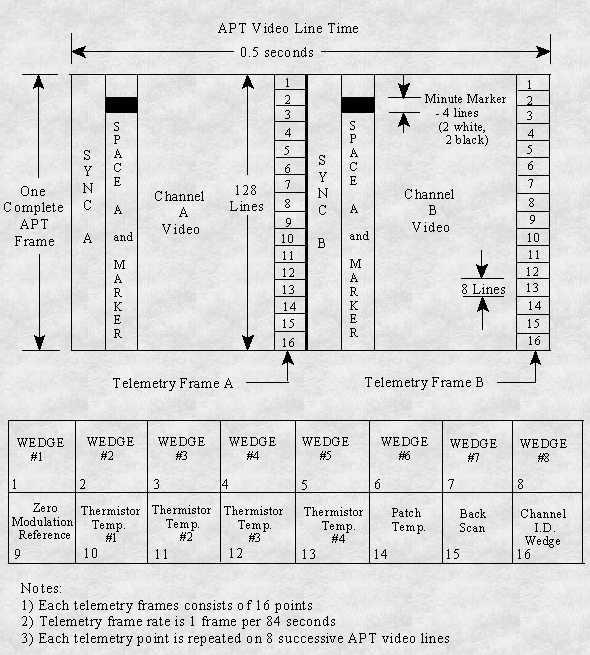
\includegraphics[width=0.5\textwidth]{apt_protocol}
\end{figure}
As shown in figure \ref{fig:aptprotocol}, data is transmitted line-by-line, one line every 0.5 seconds, each 2800px long (including metadata)~\cite[2p]{dascal2012advanced}. Lines start with a synchronisation block (832 Hz for IR, 1040 Hz for visible to distinguish the two) for the decoding software, followed by minute and space markers (the sensor briefly scans empty space turned away from earth, which shows up as pure black or white, and inserts an opposingly colored bar every minute). This is followed by the image data. At the end of each frame is the telemetry data, containing calibration data~\cite[41pp]{NOAA19building}.
\subsection{Antennas} \label{sec:NOAAantennas}
Some frequently used antenna designs are the (cheaper) turnstile antenna and the (better suited) quadrifilar antenna~\cite[45p]{NOAA19building}. The ideal polarisation is right-hand circular~\cite[44p]{NOAA19building}.\\
In our experiment, we used a different, easier design. Our antenna was a V-dipole with horizontal polarisation. This design achieves 20 dB of attenuation of the vertically polarised broadcasting stations located near the 137~MHz frequency of the POES satellites. It uses two 53.4~cm aluminium rod legs bent apart 120 degrees. They are fixed in a choc block terminal. On the other side, the shield of a coax cable is connected to one of the terminals, the inner conductor to the other~\cite{Adam15antenna}. We used standard TV coax cable, finished them with type F connectors and connected the antenna to our SDR receiver through an F-to-SMA connector. Our finished design is shown in figure \ref{fig:vdipolefinished}.
\begin{figure}
	\centering
	\caption{the antenna mounted onto a tripod with a flashlight hot-shoe clamp}
	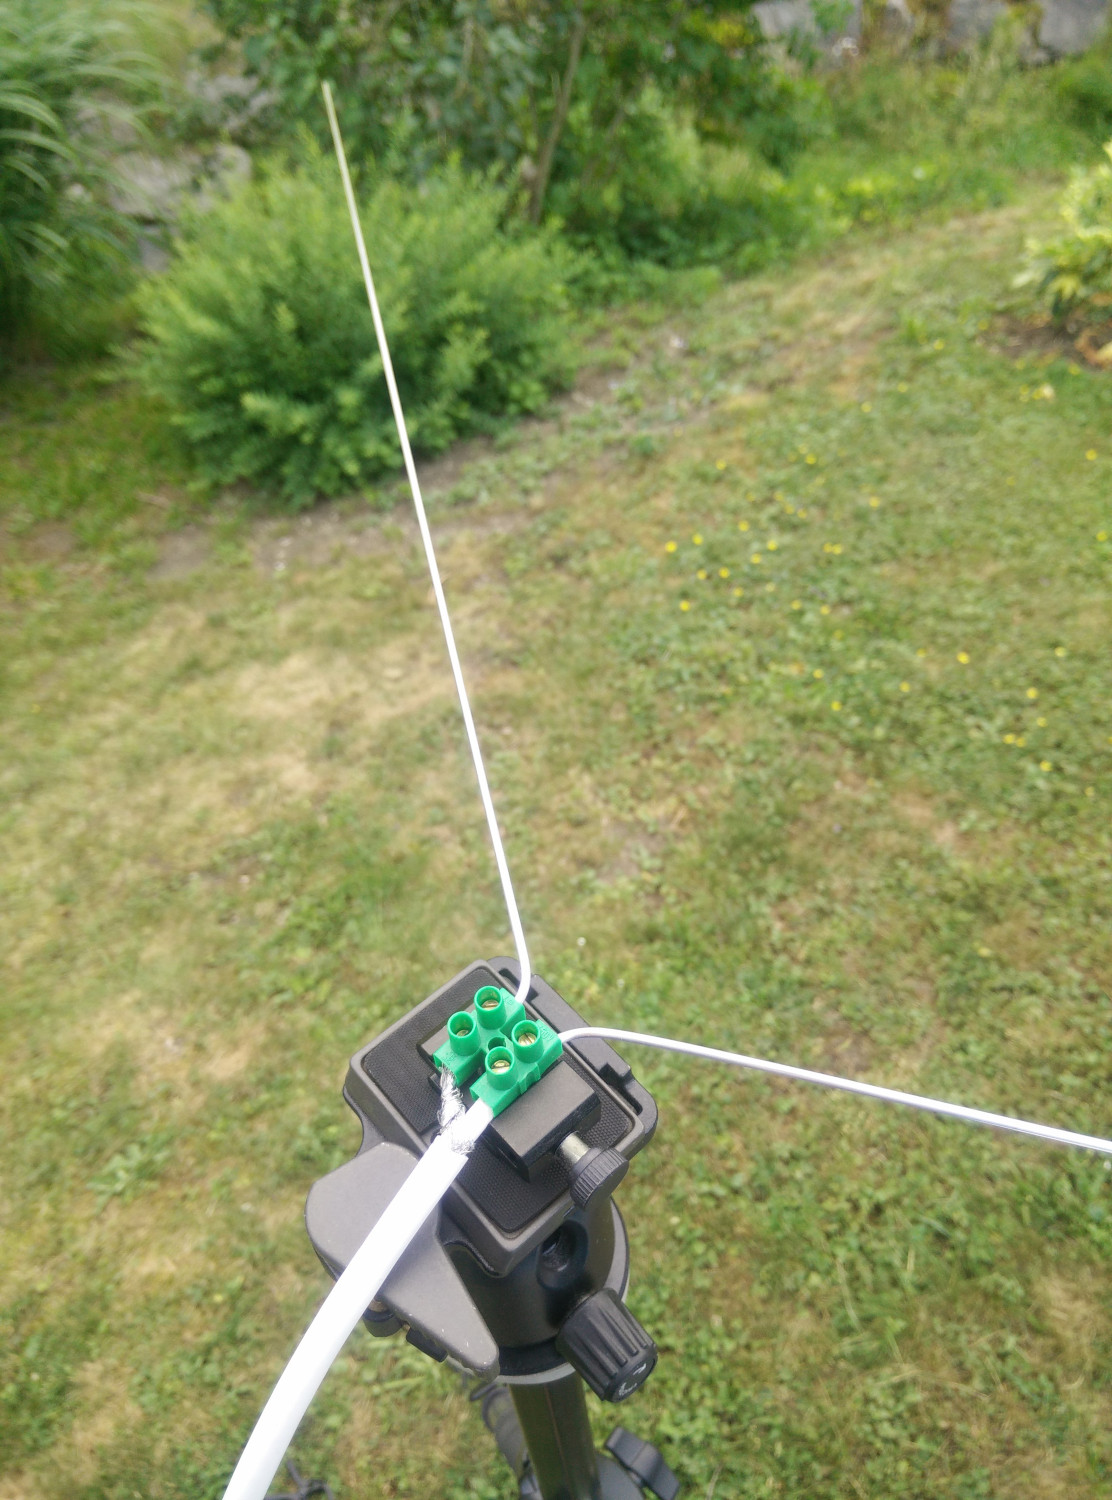
\includegraphics[width=0.5\textwidth]{v-dipole-finished} \label{fig:vdipolefinished}
\end{figure}
\subsection{Objective}
In this experiment, we attempt to receive these APT images with the mentioned inexpensive, partially self-built equipment.
\subsection{Experiment}
We performed two experiments, receiving two NOAA POES satellites, NOAA 15 and NOAA 19, at different locations.
\subsubsection{Sites}
Information about upcoming passes was sourced from \url{https://heavens-above.com/}. The first pass was NOAA 19 on 21th June 2019, 16:24 local time. The antenna was set up in a valley, and the maximum elevation of the satellite was 39 degrees, which led to a loss of signal at the beginning and end of transmission.\\
The second attempt was on an observation deck on a mountain at 750m above sea level. This reception shows more information at the extremes of the image, also due to the satellite passing directly overhead (88 degrees~\cite{heavensabove19noaa15}).\\
\subsubsection{Hardware}
We used the home-built V-dipole antenna mentioned in \ref{sec:NOAAantennas}. The SDR used was an SDRplay (RSP1A). 
\subsubsection{Software}
For receiving the signal, we used GQRX, tuned to the respective satellite frequency. Modulation was set for frequency modulation (FM). We used varying levels of gain, settling at 33.0~dB IFGR and 4.0~dB RFGR (IF = intermediate frequency/digital side, RF = radio frequency/analog side~\cite{analog07rfif}, GR = gain reduction from maximum~\cite{github18gainreduction}). Audio gain was set to -15.0~dB. The immediate bandwidth was set to approximately 60~kHz. A screenshot can be seen in figure \ref{fig:gqrx_noaa15}. The signal was recorded to a .wav-file, as shown by the pressed button in the lower right corner of figure \ref{fig:gqrx_noaa15}.\\
\balance
\begin{figure*}
	\centering
	\caption{Screenshot of GQRX while receiving NOAA 15 on 21th June, 19:16}
	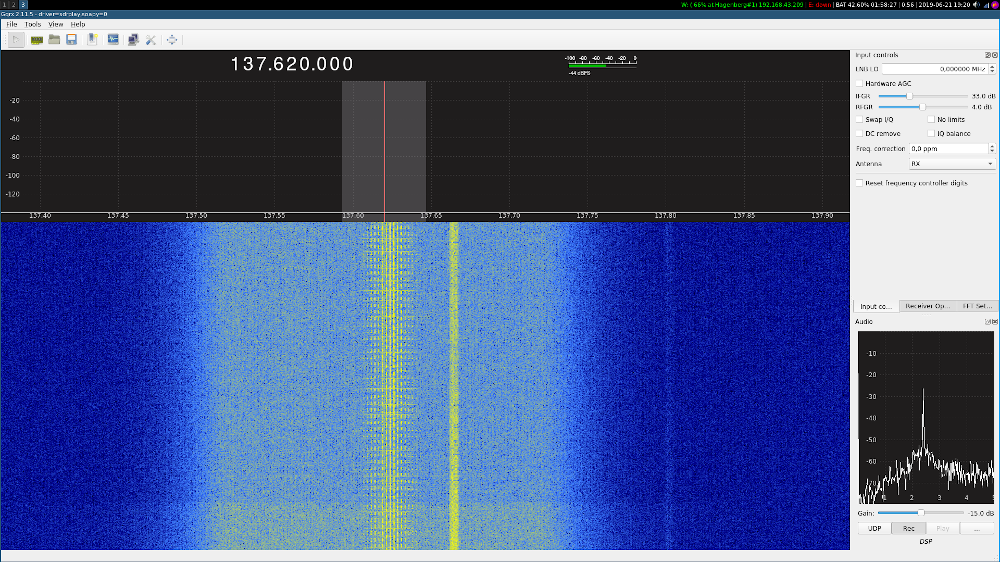
\includegraphics[width=\textwidth]{gqrx_screenshot_noaa15} \label{fig:gqrx_noaa15}
\end{figure*}
Afterwards, the image was decoded using the \textit{noaa-apt image decoder}, which is available for Windows, Linux and MacOS. A popular alternative and precedessor, \textit{WXtoIMG}, is no longer actively maintained and is only available from unofficial websites~\cite{bernardi19noaa-apt}. 
\subsubsection{Results}
As mentioned, the second recording was able to capture more information in upper/lower part of the image due to the higher vantage point and more favourable altitude of the pass. The results can be compared in figure \ref{fig:noaa19pass} and \ref{fig:noaa15pass}. The right part of figure \ref{fig:noaa19pass} (near-visible light, as the image was flipped 180 degrees due to the passing direction of the satellite) shows the Black Sea and the Crimean Peninsula in the south, and the Baltic Sea in the north. Both can be distinguished from land by their distinct darker shade of gray~\cite[42p]{NOAA19building}. Figure \ref{fig:noaa15pass} shows Great Britain, Denmark and the Netherlands, France and Sweden, Norway, Finland and Estonia. Italy and parts of Libya and Tunisia can also be seen. The position of the station is nearly exactly in the horizontal center, according to the pass data~\cite{heavensabove19noaa15}, just below a cloud formation as seen on-site.\\
The left parts show the infrared spectrum of the same area~\cite{NOAA19building}.
\begin{figure}
	\centering
	\caption{NOAA 19 on 21th June, 16:24}
	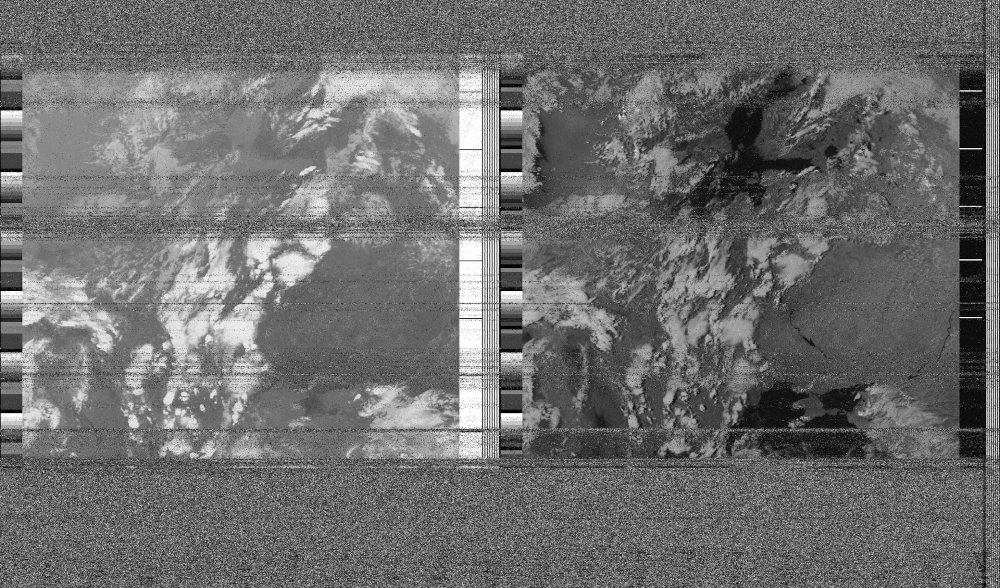
\includegraphics[width=0.5\textwidth]{noaa19_21-06-2019_1624} \label{fig:noaa19pass}
	\caption{NOAA 15 on 21th June, 19:16}
	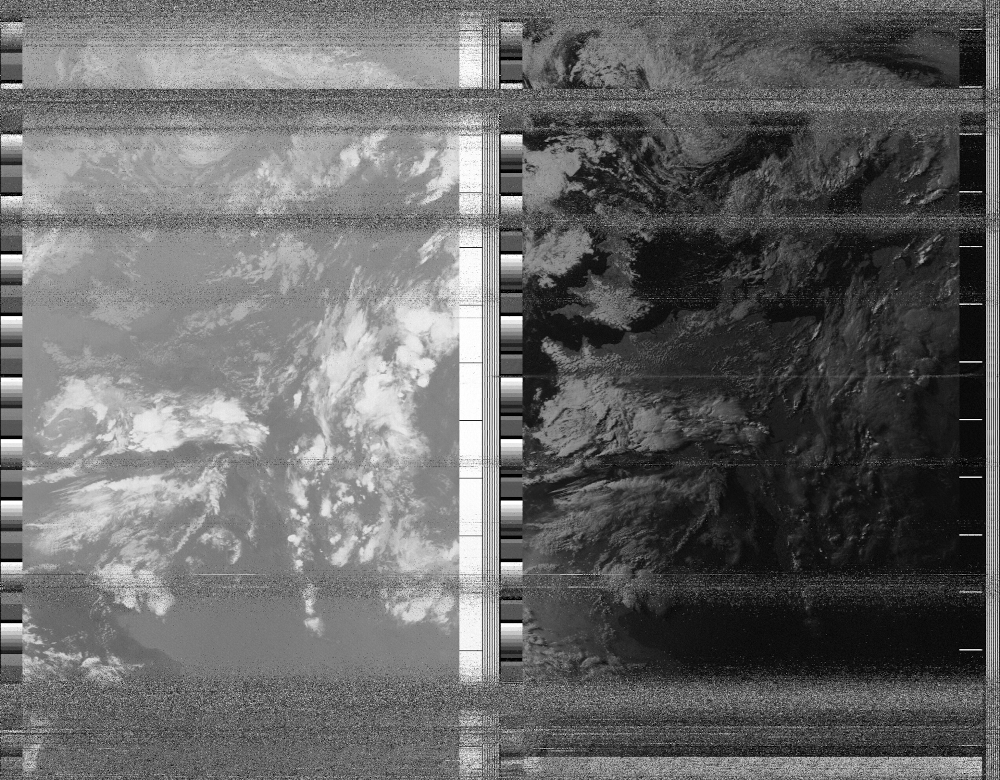
\includegraphics[width=0.5\textwidth]{noaa15_21-06-2019-1916} \label{fig:noaa15pass}
\end{figure}

\section{replay attack} %Julian
\label{replayattack}
%was ist eine replay attack?
%Beispiel Funksteckdose: Wie funktioniert die Codierung?
%wie funktioniert der workflow? HackRF + hackrf_transfer, parameter, 433 MHz Antenne

At a replay attack some radio signals are recorded at first (e.g.: unlocking a car via remote key) and transmitted at some later point in time.  If the transmitted radio signal to get some desired behaviour (e.g. switching on a remote socket) never changes, an attacker could record it with a software defined radio and transmit it afterwards at any time he/she wants to get that behaviour again. Because of this, newer cars use authentication protocols with changing codes for unlocking. \cite{verdult2015cryptanalysis}To perform this attack, whe had to know the approximate frequency range of the radio signal and to use hardware that is capable of sending and receiving radio signals within that range (e.g. HackRF One). 

\subsection{Example remote socket}
To try out the capabilities of the HackRF, we did our own replay attack on the remote control of a wireless switch unit. Most of these radio signal devices have their sending frequency written on them. This was also the case with our remote control and switch unit. On the back it said 433,92MHz (see Fig. \ref{fig:remote})

\begin{figure}[H]
	\centering
	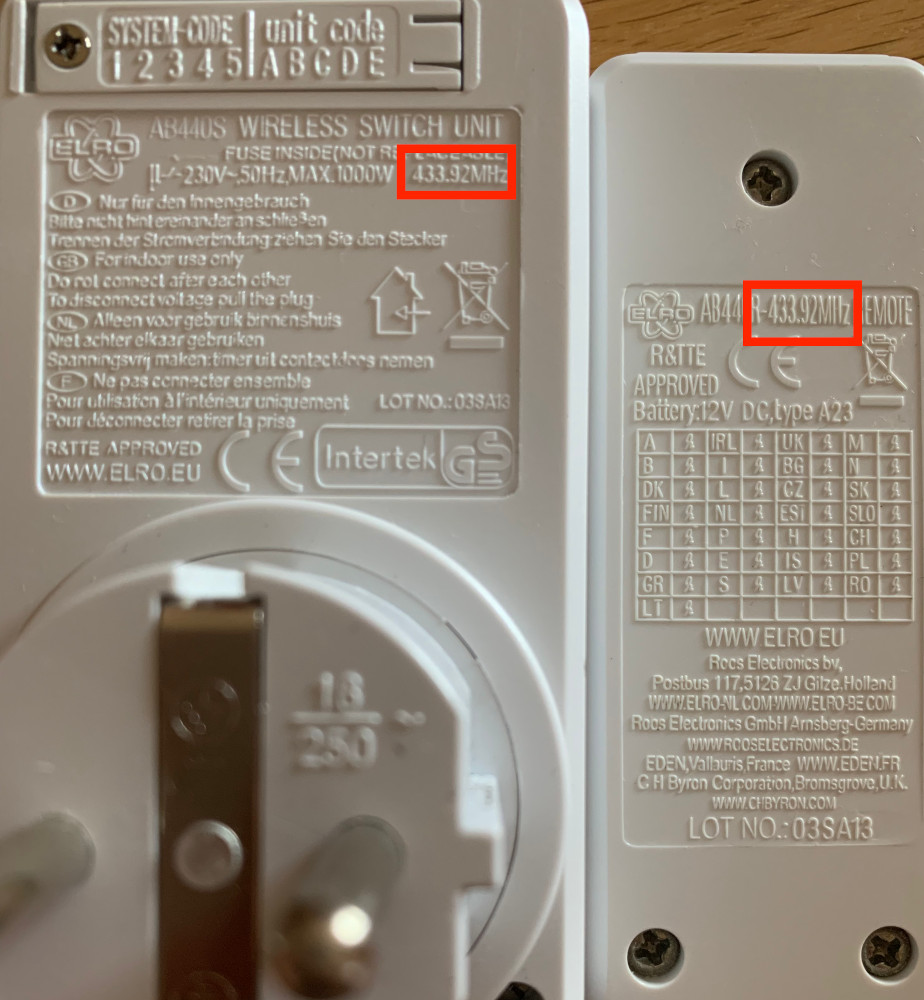
\includegraphics[width=0.5\textwidth]{remote_control_and_switch}
	\caption{Remote Control and switch unit frequency.}
	\label{fig:remote}
\end{figure}

\subsubsection{Inspecting the signal}
Based on the given frequency, we set up our RTL-SDR with the gqrx-software to inspect the sent data. When pressing the on-/off-button of the remote control we could clearly see the changes in the graphic. (see Fig. \ref{fig:remote_gqrx})


\begin{figure}[H]
	\centering
	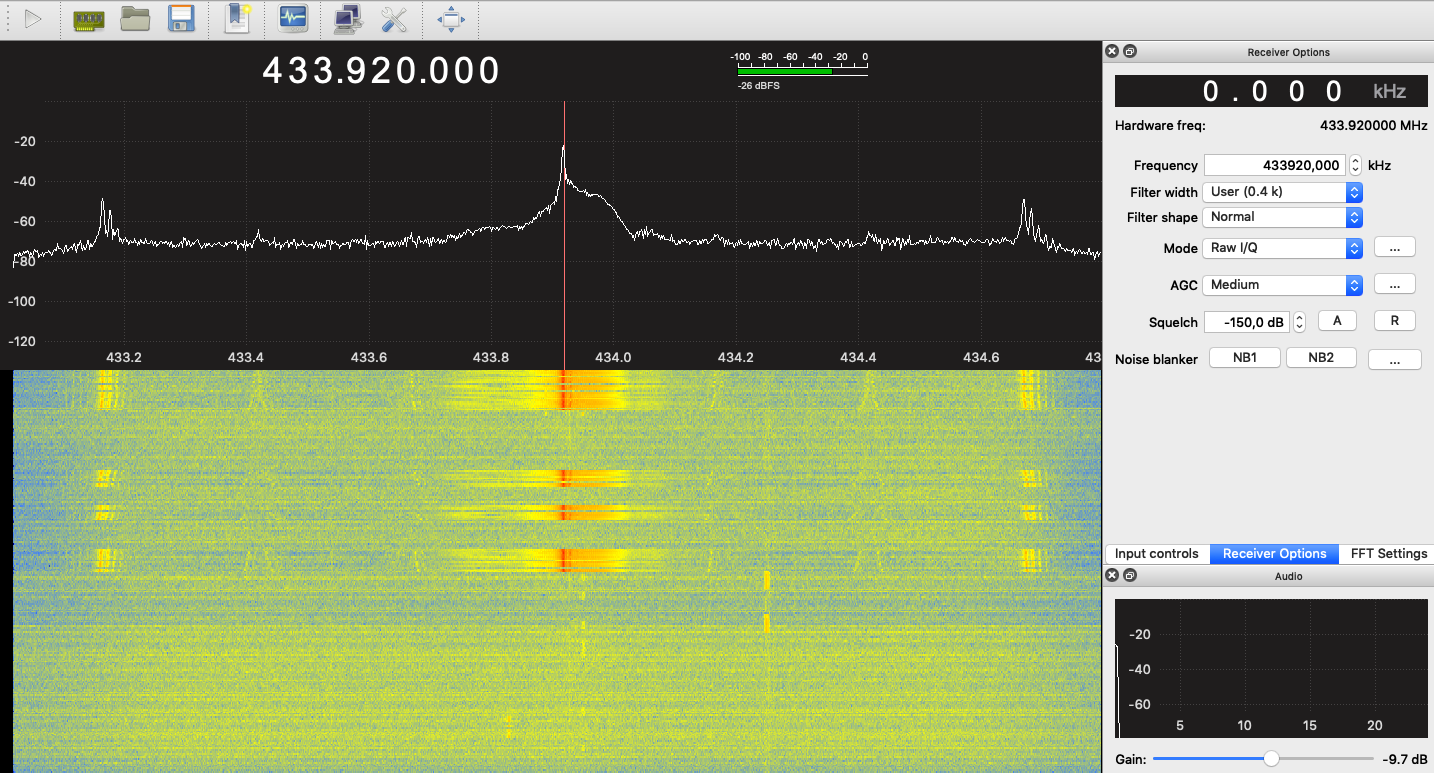
\includegraphics[width=0.5\textwidth]{gqrx_remote_control}
	\caption{Received remote control signals using gqrx.}
	\label{fig:remote_gqrx}
\end{figure}

The signal seems to have its peak at exactly 433,92MHz. There are also some side lobes noticeable (at 433,19MHz and 434,65MHz). 
\\
\subsubsection{Recording the data}
Knowing the center frequency we tried to record the data with our HackRF One.  Therefore we installed the HackRF software \cite{hackrfsoftware} using homebrew.
\begin{lstlisting}
brew install hackrf
\end{lstlisting}

To record and transmit the data with the HackRF we used the \textit{hackrf\_transfer} function. Our command was the following:
\begin{lstlisting}
hackrf_transfer -r output/received.raw -f 433920000 -l 20 -g 20 -b 2000000
\end{lstlisting}
\begin{enumerate}
	\item -r: receive
	\item -f: frequency (in Hz)
	\item -l: gain (IF) in dB
	\item -g: gain (baseband) in dB
	\item -b: baseband filter bandwidth in Hz
\end{enumerate}
\bigbreak
\subsubsection{Transmitting the data}
To transmit the edited file we again used the \textit{hackrf\_transfer} function, but now in the transmitting mode.  Our transmitting command was the following:
\begin{lstlisting}
hackrf_transfer -t output/edited.raw -f 433920000 -x 40 -b 2000000
\end{lstlisting}
\begin{enumerate}
	\item -t: transmit
	\item -f: frequency (in Hz)
	\item -x: TX gain in dB
	\item -b: baseband filter bandwidth in Hz
\end{enumerate}
Simultaneously we watched the sent data with our RTL-SDR. Through inspecting we detected that our chosen gain was too low to be detectable from the switch unit (see Fig. \ref{fig:hackrf_gqrx_g10}), so we put it up to 40dB (see  \textit{-x} in command above). That gave the signal enough power to be detected by the switch unit and to recreate the recorded behaviour. Although the replayed signal looks different than the recorded one in qgrx (see Fig. \ref{fig:hackrf_gqrx_g40}), it still works. So our replay attack was already successful.

\begin{figure}[H]
	\centering
	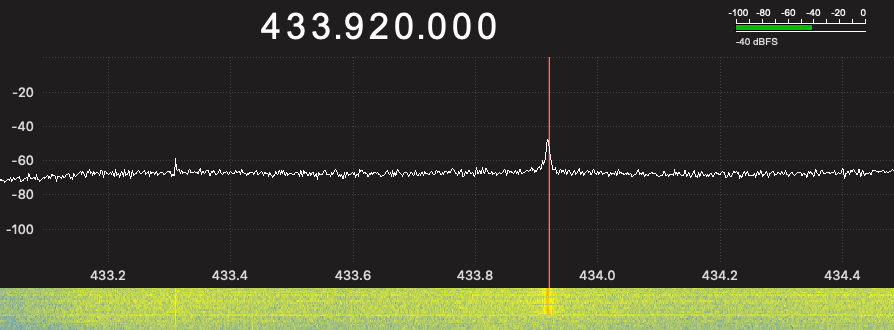
\includegraphics[width=0.5\textwidth]{gqrx_hackrf_transmission_gain10}
	\caption{The transmitted HackRF signal captured with a RTL-SDR using the gqrx software and 10dB TX gain.}
	\label{fig:hackrf_gqrx_g10}
\end{figure}

\begin{figure}[H]
	\centering
	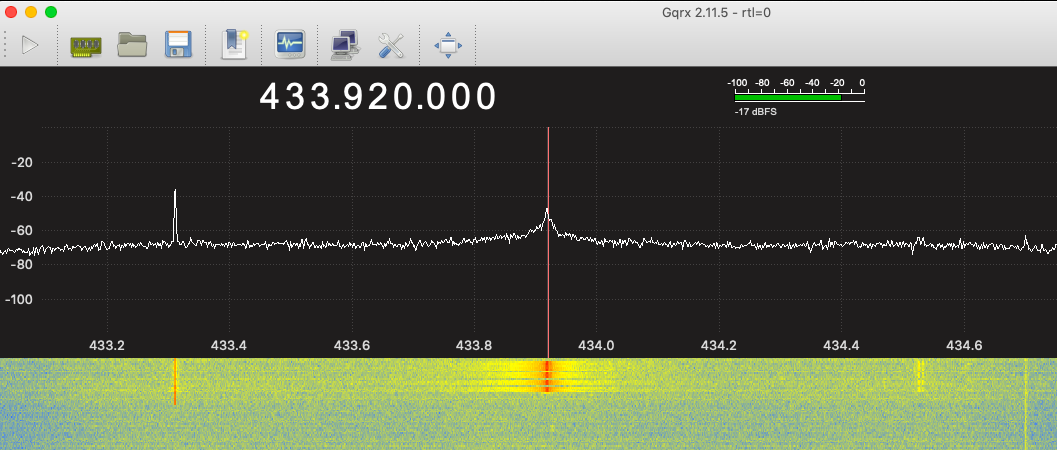
\includegraphics[width=0.5\textwidth]{gqrx_hackrf_transmission}
	\caption{The transmitted HackRF signal captured with a RTL-SDR using the gqrx software and 40dB TX gain.}
	\label{fig:hackrf_gqrx_g40}
\end{figure}
\bigbreak

\subsubsection{Cutting in Audacity}
The recorded data was very big (ca. 25MB per second of recording time), so we analysed the recorded files with the audio-editing software audacity. We imported the files into the software through \textit{file - import - rawdata} and set the import settings to the following:

\begin{enumerate}
	\item Encoding: Unsigned 16-Bit PCM
	\item Byte order: Big Endian
	\item Channels: 1 Channel (Mono=
	\item Offset: 0 Bytes
	\item Amount: 100%
	\item Sample rate: 10MHz (default of hackrf\_transfer)
\end{enumerate}
\bigbreak
After doing that we could detect, that when switching on or off there is the same signal sent periodically (see Fig. \ref{fig:audacity_on} and \ref{fig:audacity_off}). 

\begin{figure}[H]
	\centering
	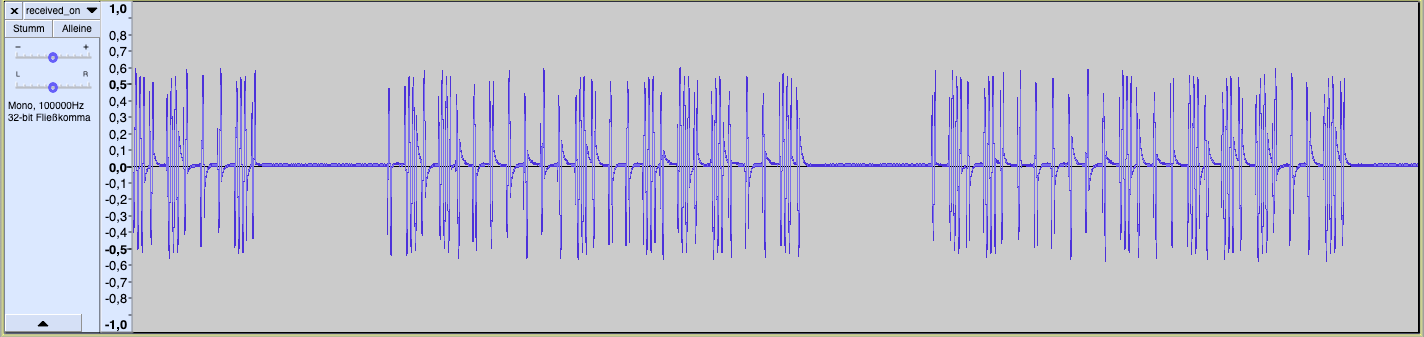
\includegraphics[width=0.5\textwidth]{audacity_received_on}
	\caption{The recorded data to switch the wireless switch unit "On", analyzed in audacity with two and a half occurrences of the periodic signal.}
	\label{fig:audacity_on}
\end{figure}

\begin{figure}[H]
	\centering
	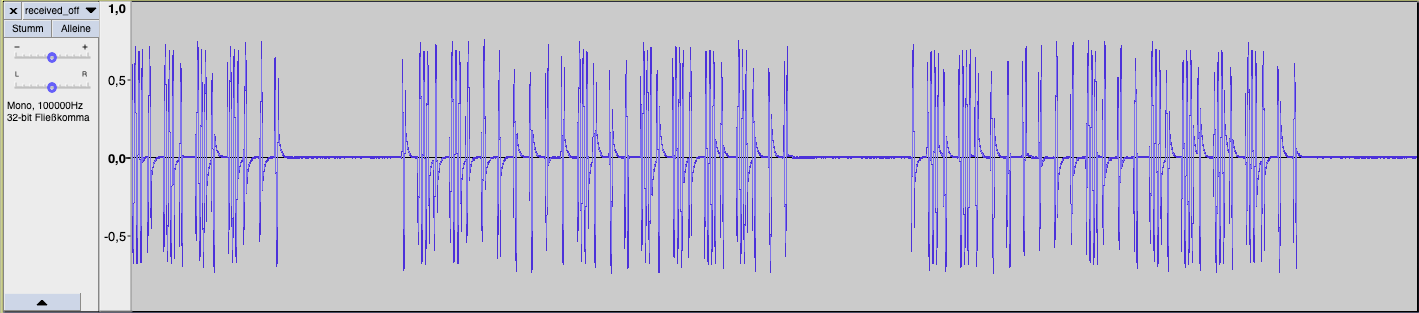
\includegraphics[width=0.5\textwidth]{audacity_received_off}
	\caption{The recorded data to switch the wireless switch unit "Off", analyzed in audacity with two and a half occurrences of the periodic signal.}
	\label{fig:audacity_off}
\end{figure}

So we could cut away most of these repetitive signals. In our case we needed at least three repetitions of the signal to switch the unit. After the cutting we exported the data again as raw file (\textit{File - export - audio export - raw (header-less) with the unsigned 16-Bit PCM encoding}) and sent it with the HackRF. In doing that we could reduce the filesize from 70MB to 2MB.

\section{Conclusion}
There are a lot of applications to use Software Defined Radio. 
%weitere Ideen:
%Radioempfang + Codierung
%rechtliche Lage: ISM-Bänder, Amateurfunklizenz
%LTE
%ship tracking
%Antennentypen: Dipol, Yagi, Patch, Parabol, ...

\bibliographystyle{IEEEtran}
\bibliography{references}

\end{document}
